\subsection{Seismic attributes}
\label{subsec:seismic-attributes}

Seismic attributes are quantitative measures derived from seismic data describing various subsurface geology aspects.
Over the past few decades, seismic attributes have become indispensable tools in the exploration and production of hydrocarbons, mineral resources, and the management of geohazards.
They have significantly contributed to the understanding of complex geological settings and have improved the accuracy of reservoir characterization and prediction.

Seismic data, obtained through controlled seismic sources and an array of receivers, is used to create images of the subsurface geology.
The acquired data is processed and interpreted to reveal geological features, such as faults, fractures, and rock properties.
However, seismic data can be challenging to interpret due to the subsurface geology's complex nature and seismic imaging techniques' limitations.

The evolution of seismic attributes is explored by Barnes and Arthur~\cite{barnes2001seismic}, Chopra \etal~\cite{chopra2005seismic}, Fawad \etal~\cite{fawad2020seismic}, and Taner and Turhan~\cite{taner2001seismic}.
This concept was first introduced in the late 1970s to enhance the interpretation of seismic data.
Since then, the field has experienced significant advancements, driven by the growth in computational power and the development of innovative seismic processing and interpretation techniques.

To illustrate the usage of seismic attributes, Figure~\ref{fig:seismic-complex-attr} shows a sample of two complex seismic attributes derived from the amplitude of a sample seismic data.
The amplitude envelope, illustrated by Figure~\ref{fig:seismic-envelope}, highlights the presence of a potential hydrocarbon reservoir.
Figure~\ref{fig:seismic-inst-phase} shows the instantaneous phase of the seismic data, which defines the phase of the seismic wavelet at each sample.

\begin{figure}[htb!]
    \captionsetup[subfigure]{justification=centering}
    \centering

    \subfloat[][Amplitude (raw data)]{
        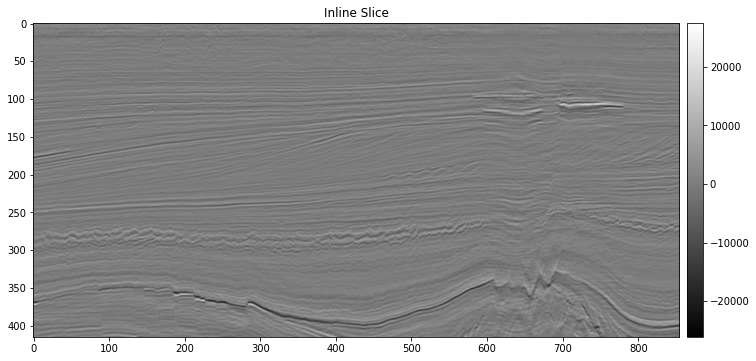
\includegraphics[height=4cm]{images/seismic-amplitude.png}
        \label{fig:seismic-raw-data}
    }
    
    \subfloat[][Amplitude envelope (the red arrow highlights a possible hydrocarbons reservoir)]{
        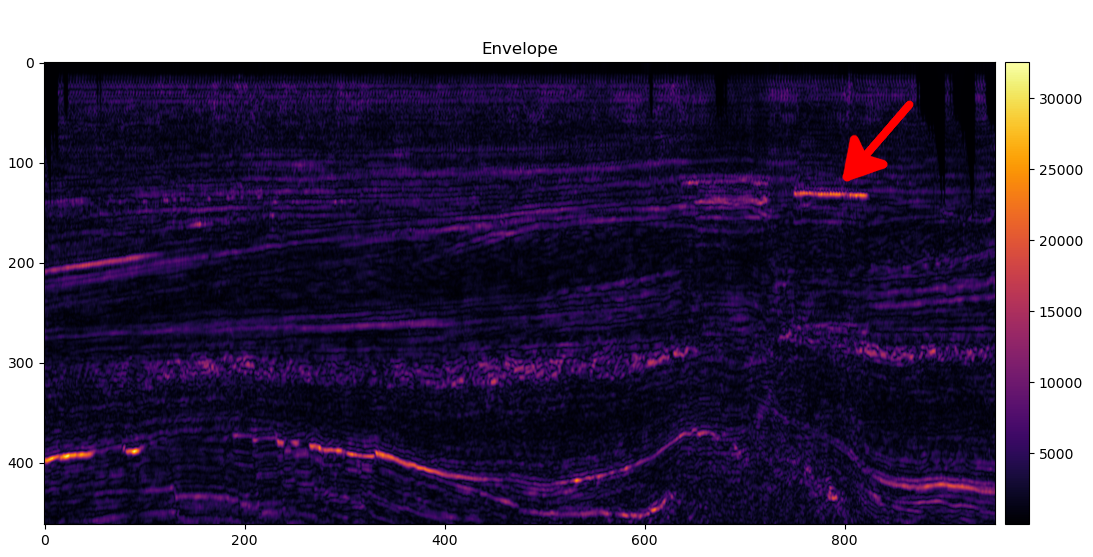
\includegraphics[height=4cm]{images/seismic-envelope.png}
        \label{fig:seismic-envelope}
    }
    \subfloat[][Instantaneous phase]{
        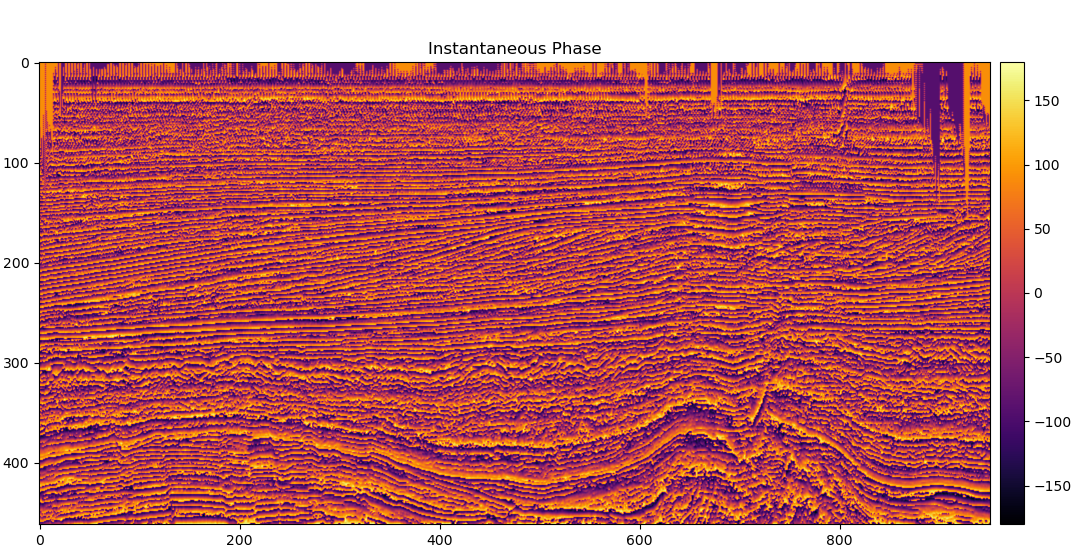
\includegraphics[height=4cm]{images/seismic-inst-phase.png}
        \label{fig:seismic-inst-phase}
    }

    \caption{sample of two complex seismic attributes derived from the amplitude to the inline}
    \label{fig:seismic-complex-attr}
\end{figure}

As explained in the previous example, integrating seismic attributes into the interpretation workflow allows geoscientists to extract valuable information from seismic data more efficiently.
Seismic attributes can be combined with other data, such as logs and geological models, to understand subsurface geology comprehensively.
Furthermore, advanced machine learning and data analytics techniques have enabled the development of multi-attribute analysis, which involves the simultaneous examination of multiple attributes to identify patterns and relationships that may not be apparent when considering individual attributes.

Seismic attributes play a crucial role in analyzing and interpreting seismic data by providing quantitative measures of subsurface geology.
They enhance the understanding of complex geological settings, improve reservoir characterization, and aid in the prediction of subsurface resources.
As the field continues to evolve, integrating seismic attributes with other data sources and advanced computational techniques will further advance the state of knowledge in the field and enable more accurate and efficient exploration and production efforts.
